\documentclass[12pt,letterpaper,final]{report}
\usepackage[utf8]{inputenc}
\usepackage{amsmath}
\usepackage{amsfonts}
\usepackage{amssymb}
\usepackage{amsthm}
\renewcommand\qedsymbol{$\blacksquare$}
\usepackage{enumerate}
\usepackage{hyperref}
\usepackage{pdfpages}
\usepackage{graphics}
\usepackage{graphicx}
\usepackage{tikz}
\usepackage{tikz-qtree}
\usetikzlibrary{automata,arrows, arrows.meta, positioning}
\usepackage[
  backend=biber,
  style=authoryear,
  sorting=nyt          % sort by name, year, title
]{biblatex}
\addbibresource{references.bib}

% \author{Marius Zimand}
\author{Jonathan Llovet}

\begin{document}

\fbox{
  \vbox{
    \begin{flushleft}
      Jonathan Llovet \\  % authors' names
      COSC 417 \\  %class
      2026-02-26, 11:59 PM (EST) \\  % date
    \end{flushleft}
    \center{\Large{\textbf{Assignment 3}}}
    %\end{mdframed}
  } % end vbox
} % end fbox
\vline

Do without turning in anything the following exercises regarding regular expressions from the textbook: 1.19, 1.20, 1.21  (Some of them have solutions in the book; still try to do them before checking the solution. Some of this exercises will show up in quizzes).


Read Examples 1.73 - 1.77  from the textbook, which use the Pumping lemma to show that certain languages are not regular. (Some of these exercises will show up in quizzes and exams).

Do (or at least sketch the solutions) without turning in anything the following exercises from the textbook: 1.4 (a-d), 1.5 (a-d), 1.6(a-d), 1.7(a-d).

\medskip

Do and turn in the following exercises.

\pagebreak

1.  Exercise 1.16  - page 86. Use the method shown in class and which is also in the textbook in Example 1.41, page 56.

  {\bf Part A:}

\begin{center}
  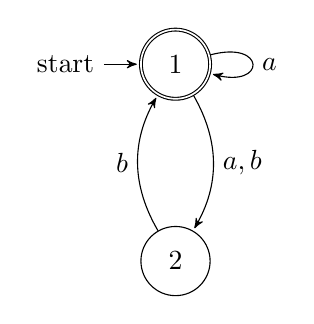
\begin{tikzpicture}[>=stealth',shorten >=1pt,auto,node distance=2.5cm]

    \node[initial, state, accepting] (1) {$1$};
    \node[state] (2) [below of=1] {$2$};

    \path[->]
    (1) edge [loop right] node[right] {$a$} (1)
    (1) edge [bend left] node[right] {$a,b$} (2)
    (2) edge [bend left] node[left] {$b$} (1)
    ;
  \end{tikzpicture}
\end{center}

The DFA that corresponds to the NFA above is defined as follows:

\begin{align*}
  A = \Big( & Q = \{\emptyset, \{1\}, \{2\}, \{1,2\}\},       \\
            & \Sigma = \{a,b\},                               \\
            & \delta \text{ (as defined in the table below)}, \\
            & q_0 = \{1\},                                    \\
            & F = \{\{1\}, \{1,2\}\} \Big)
\end{align*}

\begin{center}
  $\delta =$
  \begin{tabular}{|c|c|c|}
    \hline
    state       & $a$         & $b$         \\
    \hline
    $\emptyset$ & $\emptyset$ & $\emptyset$ \\
    $\{1\}$     & $\{1,2\}$   & $\{2\}$     \\
    $\{2\}$     & $\emptyset$ & $\{1\}$     \\
    $\{1,2\}$   & $\{1,2\}$   & $\{1,2\}$   \\
    \hline
  \end{tabular}
\end{center}


\medskip

2.	Give regular expressions for each of the following languages over the alphabet $\{0,1\}$:
\medskip

(a)	$\{w \in  \{0, 1\}^* \mid \mbox{ $w$ begins with a $1$ and ends with a $1$}\}$
\[
  1(1 \cup 0)^*1 \cup 1
\]

(b)	$\{w  \in \{0, 1\}^*  \mid \mbox{ $w$ has length at least $3$ and its 2nd symbol is a $0$}\}$
\[
  (1 \cup 0)0(1 \cup 0)^+
\]

(c)	$\{w  \in \{0, 1\}^*  \mid \mbox{ $w$ does not contain $01$} \}$.
\[
  1^*0^*
\]

\medskip

\pagebreak
In the following $3$ exercises, use the Pumping Lemma or the closure properties of regular languages to prove that the  corresponding languages are not regular.
\medskip

3. 	$B=\{w  \in \{0, 1\}^* \mid \mbox{ the number of 0s in $w$ is two times the number of 1s in $w$}\}$.
\smallskip

By the pumping game, based on the contrapositive of the pumping lemma:
\[
  \begin{array}{llll}
    \text{I (Us):}   & \text{Let } s = 0^{2p}1^p &  & \text{satisfying } \vert s \vert \ge p                     \\
    \text{II (Adv):} & \text{Let }s =  xyz       &  & \text{such that: } y \not = \epsilon, \vert xy \vert \le p \\
    \text{III (Us):} & \text{Take } i = 2        &  & \text{then } xy^2z \not \in B                              \\
  \end{array}
\]

This consequence is because with $i=2$, there will be more than $2p$ $0$'s, but only $p$ $1$'s, which does not satisfy the condition for inclusion in $B$.

\medskip

4. 	$A = \{0^{n!} \mid n >= 0 \}$ (Reminder: $n! = 1  \cdot 2 \cdot  \ldots \cdot  n$)
\medskip

By the pumping game, based on the contrapositive of the pumping lemma:
\[
  \begin{array}{llll}
    \text{I (Us):}   & \text{Let } s = 0^{p!}                                        &  & \text{satisfying } \vert s \vert \ge p                     \\
    \text{II (Adv):} & \text{Let }s =  xyz                                           &  & \text{such that: } y \not = \epsilon, \vert xy \vert \le p \\
    \text{III (Us):} & \text{Take } i = 0. \text{ Let $x = \epsilon, z = \epsilon$.} &  & \text{then } xy^0z \not \in A                              \\
  \end{array}
\]

This works by pumping down. $xy^0z \not \in A$ because $n! \ge 1$, but $\vert xy^0z\vert = 0$, which means $xy^0z$ does not satisfy the condition for inclusion in $A$.

\medskip

5. 	$C = \{0^m1^n  \mid  m \not= n \}$ (Note: This is an example where the pumping lemma is difficult to use.   It is much easier to use the closure properties of regular languages.)

{\bf Proof by contradiction:} We wish to prove that $C$ is not regular. Assume to the contrary that $C$ is regular. Because regular languages are closed under complement, $C_1 = C^c$ is regular. This includes all strings that are not in $C$ over the alphabet $\{0,1\}$. Additionally, let $C_2 = \{0^m1^n \mid m, n \ge 0\}$. These are all the strings that are in form of some number of $0$'s followed by some number of $1$'s. Then let $C_3 = C_1 \cap C_2$. Because regular languages are closed under intersection, therefore $C_3$ is also regular. This is the language of strings that have some $0$'s followed by some $1$'s that are not in $C$. That is, $C_3 = \{0^m1^n  \mid  m = n \}$. But this language we know to be irregular. Because the complement and intersection operations on a language preserve its regularity, this means that if $C$ were regular, then $C_3$ would also be regular. However, we found that $C_3$ is not regular, which contradicts our assumption. Therefore $C$ is not regular.
\medskip

% {\small
%   (Some hints for exercises 3-5: If you use the Pumping Lemma, present how Player 1 can win the game in 3 moves. Remember that in the first move, Player 1 must choose a string that has length at least p, and p is an arbitrary number. In step 3 you must show that Player 1 has a winning move, for \emph{any} move of Player 2 in the second move.

%   Exercise 3 is similar to Example 1.73 in the textbook (which we also did in class), Exercise 4 is similar to Example 1.76 in the textbook.

%   If you use the closure properties for Exercise 5, you need to transform (using the operations of union, intersection, complementation, concatenation, and star) the language $C$ into $L_1$, and then $L_1$ into $L_2$, and so on till you reach a language that you know already is not regular.
%   This implies that the initial language $C$ is also not regular.)
% }
\medskip

6. Show that if $A$ is a regular language, then $A_{even} = \{x \in A \mid |x| \textrm{ is even} \}$ is also regular. \emph{Hint:} $A_{even}$ is the subset of $A$ containing all strings in $A$ with even length. You can use a closure property.

Consider the language $B$ that is represented by the DFA below:

\begin{center}
  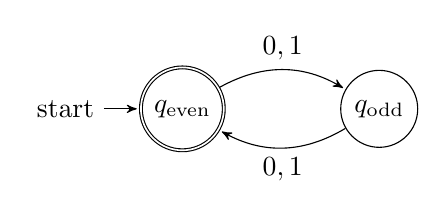
\begin{tikzpicture}[>=stealth',shorten >=1pt,auto,node distance=2.5cm]

    \node[initial, state, accepting] (0) {$q_{\text{even}}$};
    \node[state] (1) [right of=0] {$q_{\text{odd}}$};

    \path[->]
    (0) edge [bend left] node[above] {$0,1$} (1)
    (1) edge [bend left] node[below] {$0,1$} (0)
    ;
  \end{tikzpicture}
\end{center}

Since $B$ is represented by a DFA, it is regular. The language $B$ can also be expressed: $\{x \in {\{0,1\}}^* \mid \vert x \vert \text{ is even}\}$. For any alphabet used for $A$, an analogous DFA can be constructed for $B$ by adding edges for the corresponding characters in the alphabet. Furthermore, the language $A_1 = A \cap B$ is regular, because of the closure of regular languages over intersection. But $A_1 = \{x \in A \mid |x| \text{ is even} \}$. This, however, is the same as $A_{even}$. Therefore, since $A_1$ is regular by the closure over intersection of regular languages and $A_1 = A_{even}$, $A_{even}$ is also regular.

\bigskip


%The next problem is \textbf{Extra Credit}.  It is optional. If you choose to do this part, you need to do it alone (without a partner) and turn it separately in class. Write on top of it: "Assignment 3 -Extra Credit" and your name.
%\medskip

7.  Find the mistake in the following ``proof" that shows that the language $L = a^* b^*$ (formally, $L$ is the language denoted by the regular expression $a^* b^*$) is not regular (which obviously is false).
\medskip

\emph{``Proof" that $L$ is not regular}.

Suppose $L$ is regular, and let $p$ be the pumping length for $L$. We play the Pumping Game for $L$.
\medskip

I. We choose $s = a^{p/2} b^{p/2}$ if $p$ is even. If $p$ is odd, we take $s = a^{(p+1)/2} b^{(p+1)/2}$ .
\smallskip

II. The adversary breaks $s = xyz$ so that $y=ab$.
\smallskip


III. We take $i=2$. We have won the game: $xyyz$ is not in $L$ because it has as a subword $abab$ which is not allowed for strings in $L$.
\medskip

Since we have won the Pumping Game, it follows that $L$ is not regular.

\emph{End of ``Proof''}

\end{document}
